\documentclass[aspectratio=43]{beamer}
\usepackage[latin1]{inputenc}
\usepackage{amsmath}
\usepackage{amsfonts}
\usepackage{amssymb}
\usepackage{makeidx}
\usepackage{graphicx}
\usepackage{array}

% Customization
\mode<presentation>{
\usetheme{CambridgeUS}
\usecolortheme{dolphin}
\setbeamertemplate{navigation symbols}{}
}

%\setbeamertemplate{footline}[frame number]

%TikZ diagrams
\usepackage{tikz}
\usetikzlibrary{patterns}
\usetikzlibrary{arrows,shapes}
\usetikzlibrary{shapes.multipart}
\usetikzlibrary{trees}
\usetikzlibrary{shapes.geometric}
\usetikzlibrary{matrix,arrows}
\usetikzlibrary{positioning}
\usetikzlibrary{calc,through}
\usetikzlibrary{decorations.pathreplacing}
\usepackage{pgffor}

% Define colors
\definecolor{darkgreen}{rgb}{0.0, 0.5, 0.13}
\definecolor{darkblue}{rgb}{0.0, 0.0, 0.55}
\definecolor{darkred}{rgb}{0.55, 0.0, 0.0}

% For using TikZ
\usetikzlibrary{decorations.pathmorphing}
\usetikzlibrary{decorations.markings}
\tikzset{
	vector/.style={decorate, decoration={snake,amplitude=3pt}, draw},
	gluon/.style={decorate, decoration={coil,amplitude=2.5pt},draw},
	provector/.style={decorate, decoration={snake,amplitude=2.5pt}, draw},
	antivector/.style={decorate, decoration={snake,amplitude=-2.5pt}, draw},
	fermion/.style={draw=black, postaction={decorate},
		decoration={markings,mark=at position .55 with {\arrow[draw=black,thick]{>}}}},
	fermionbar/.style={draw=black, postaction={decorate},
		decoration={markings,mark=at position .55 with {\arrow[draw=black,thick]{<}}}},
	fermionnoarrow/.style={draw=black},
	gluon/.style={decorate, draw=black,
		decoration={coil,amplitude=2.5pt, segment length=3pt}},
	gluon2/.style={decorate, draw=black,
		decoration={coil,amplitude=1.75pt, segment length=2.75pt}},
	scalar/.style={dashed,draw=black, postaction={decorate},
		decoration={markings,mark=at position .55 with {\arrow[draw=black]{>}}}},
	scalarbar/.style={dashed,draw=black, postaction={decorate},
		decoration={markings,mark=at position .55 with {\arrow[draw=black]{<}}}},
	scalarnoarrow/.style={dashed,draw=black},
	electron/.style={draw=black, postaction={decorate},
		decoration={markings,mark=at position .55 with {\arrow[draw=black]{>}}}},
	bigvector/.style={decorate, decoration={snake,amplitude=4pt}, draw},
}

% Blocks
\tikzstyle{block} = [draw, rectangle, minimum height = 3em, rounded corners, minimum width = 4em]
\tikzstyle{block2} = [draw, rectangle, minimum height = 3em, rounded corners, minimum width = 7em]
\tikzstyle{circle} = [draw, circle, radius = 1.5]
\tikzstyle{arrow} = [thick,->]
%************************************************************************************************************

% Title and author
\title[Fast predictions for Higgs production]{Fast predictions for Higgs production}
\author{\textbf {Jes\'us Urtasun Elizari}}
%\institute{\textbf {University of Milan}}
\date{Milan, September 2020}

\begin{document}

% Front slide
\begin{frame}

	%\maketitle
	\vspace{1.0 cm}
	
	\center{\color{blue}HTurbo: Fast predictions for Higgs production at the LHC}
	
	\vspace{0.25 cm}
	\center{Jes\'us Urtasun Elizari}
	\center{PhD seminar - Milan, September 2020}

	\begin{figure}
		\minipage{1\textwidth}
		
\includegraphics[width = 3.0 cm]{plots/unimi.png}
		\hfill
		
\includegraphics[width = 3.0 cm]{plots/n3pdf.png}
		\hfill
		
\includegraphics[width = 3.0 cm]{plots/erc.png}
		\endminipage
	\end{figure}

	\vspace{1.0 cm}
	
	{\scriptsize \color{blue} This project has received funding from the European Union$'$s Horizon 2020 research and innovation program under grant agreement No 740006.}

\end{frame}

% Introduction
\begin{frame}

	\frametitle{Outline}
	
	\begin{enumerate}
		\item {\color{blue}QCD in a nutshell}
		\begin{itemize}
			\item Factorization in QCD
			\item Partonic cross section
			\item Perturbative QCD
		\end{itemize}
		\item {\color{blue}Resummation in QCD}
		\begin{itemize}
			\item Higher order corrections
			\item Resummation of $q_{\perp}$
		\end{itemize}
		\item {\color{blue}HTurbo}
		\begin{itemize}
			\item Higgs production at the LHC: HRes and HqT
			\item HTurbo: Fast predictions for Higgs production
			\item Results $\&$ Conclusions
		\end{itemize}
	\end{enumerate}
	
\end{frame}

% QCD in a nutshell
\begin{frame}

\center{\color{blue}QCD in a nutshell}

\end{frame}

% Parton Distribution Functions
\begin{frame}

	\frametitle{QCD in a nutshell}
	\framesubtitle{Address nuclear structure}
	
	\begin{figure}
		\minipage{0.5\textwidth}
		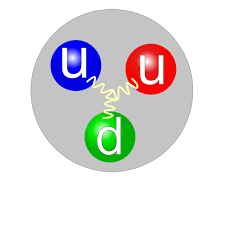
\includegraphics[width = 0.5\linewidth]{plots/proton.png}
		\endminipage\hfill
		\minipage{0.5\textwidth}
		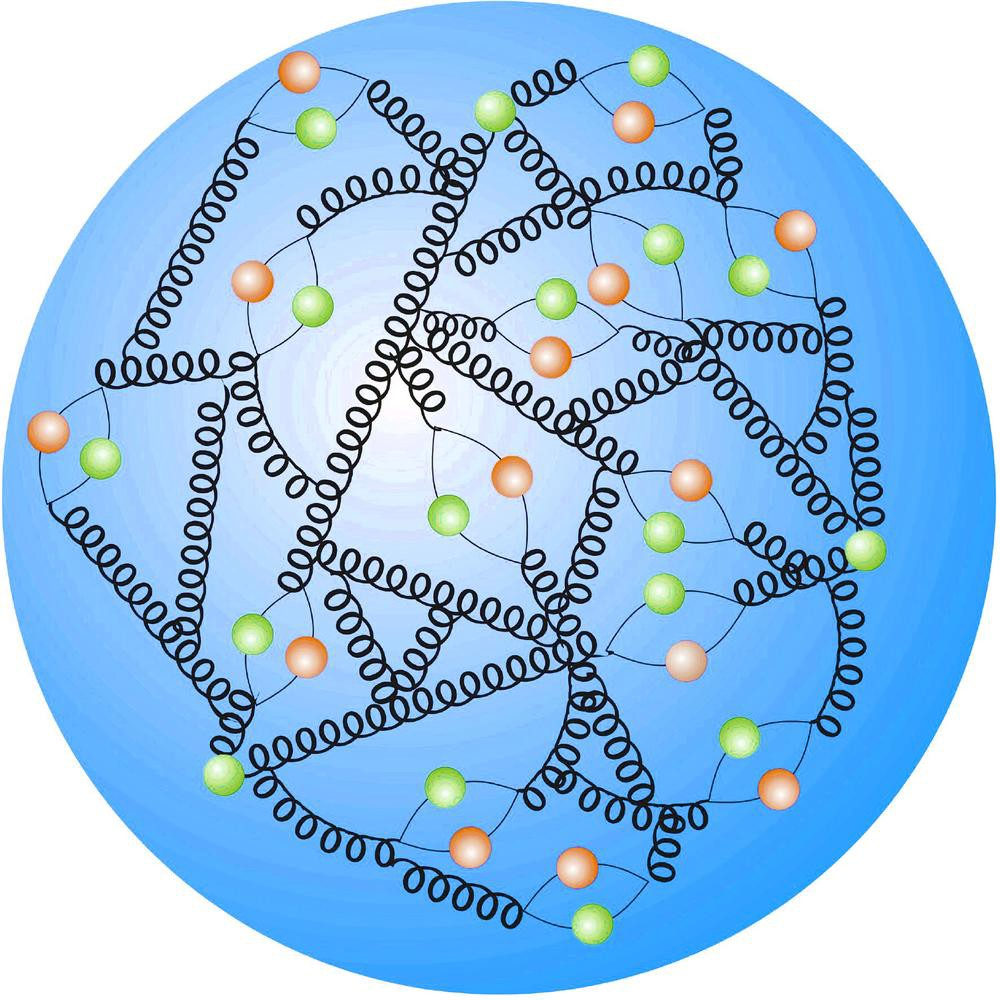
\includegraphics[width = 0.4\linewidth]{plots/proton2.jpg}
		\endminipage
	\end{figure}
	
	\begin{itemize}
		\item Hadrons made of partonic objects $\longrightarrow$ non perturbative physics
		\item Smash two hadrons to explore internal structure $\longrightarrow$ LHC physics
		\item Compute cross section is a {\color{red}hard problem} $\longrightarrow$ {\color{blue}QCD Factorization}
	\end{itemize}

\end{frame}

% Factorization theorem I
\begin{frame}

	\frametitle{QCD in a nutshell}
	\framesubtitle{Factorization theorem}

	\begin{figure}
		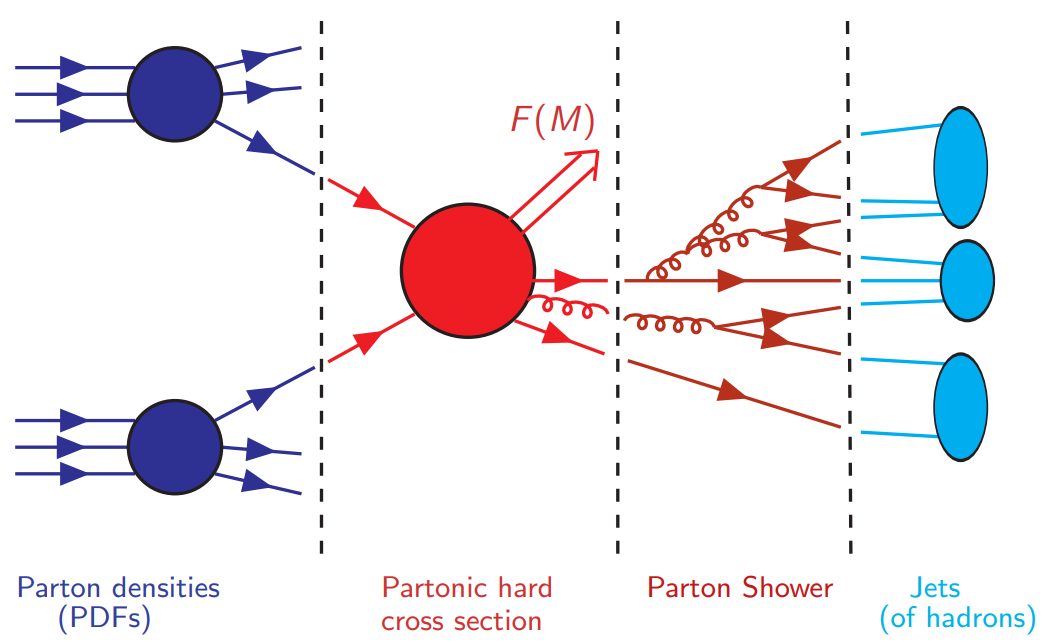
\includegraphics[width = 7 cm]{plots/factorization_1.png}
	\end{figure}
	
	Factorization in QCD $\longrightarrow$ Convolute the {\color{blue}PDFs} with the partonic ${\color{red}\hat{\sigma}_{\alpha\beta}^{\textrm{F}}}$
	
	\begin{equation}
		\sigma^{\textrm{F}}(p_{1}, p_{2}) =
		\int_{0}^{1} dx_{1} dx_{2} \; {\color{blue} f_{\alpha}(x_{1}, \mu_{F}^{2}) \ast f_{\beta}(x_{2}, \mu_{F}^{2})}
		\; \ast \;  
		{\color{red}\hat{\sigma}^{\textrm{F}}_{\alpha \beta}(x_{1}p_{1}, x_{2}p_{2}, \alpha_{s}(\mu_{R}^{2}), \mu_{F}^{2})} \nonumber
	\end{equation}

\end{frame}

% Partonic cross section
\begin{frame}
	
	\frametitle{QCD in a nutshell}
	\framesubtitle{Partonic cross section}
	
	\begin{figure}
		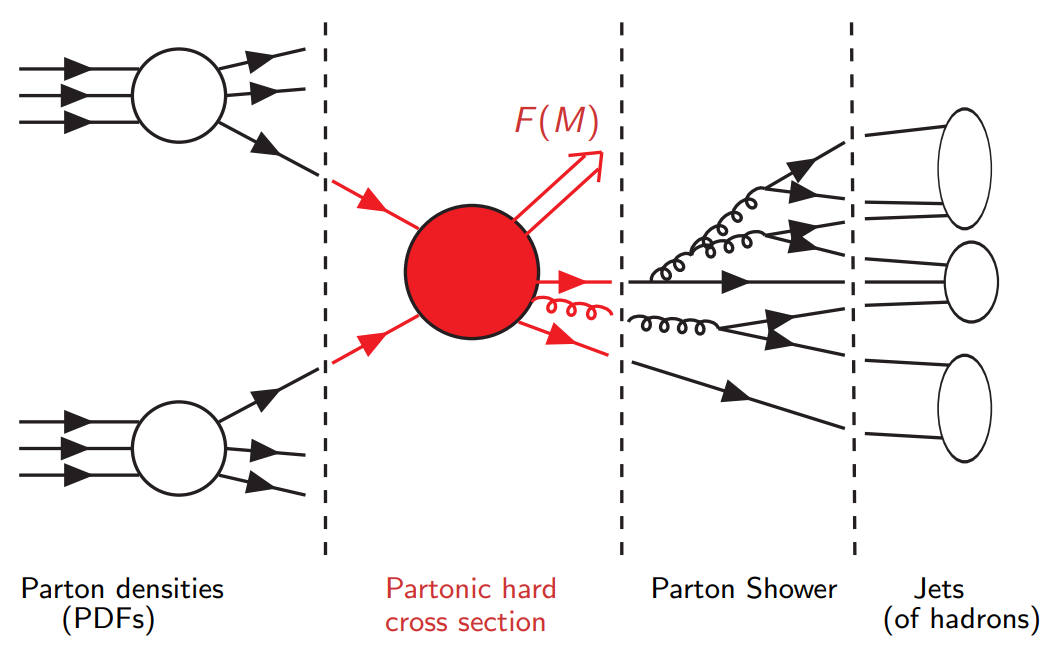
\includegraphics[width = 7 cm]{plots/factorization_2.png}
	\end{figure}
	
	\begin{itemize}
		\item {\color{blue}PDFs} ${\color{blue} f_{\alpha}(x_{i}, \mu_{F}^{2})}$ absorb the non perturbative effects, evaluated at $\mu_{F}$
		\item Partonic {\color{red}$\hat{\sigma}^{\textrm{F}}_{\alpha \beta}$} can be computed as perturbative series in $\alpha_{s}$
	\end{itemize}
	
\end{frame}

% Perturbative QCD
\begin{frame}

	\frametitle{QCD in a nutshell}
	\framesubtitle{Perturbative QCD}
	
	\begin{columns}
		
		\column{0.45\textwidth}
		
		\begin{itemize}
			\item Born cross section as LO value of a perturbative series
			\item $\sigma^{(1)}, \sigma^{(2)}, \sigma^{(3)}$ are the NLO, NNLO, N3LO corrections
		\end{itemize}
		
		\column{0.45\textwidth}
		\begin{figure}[!htb]
			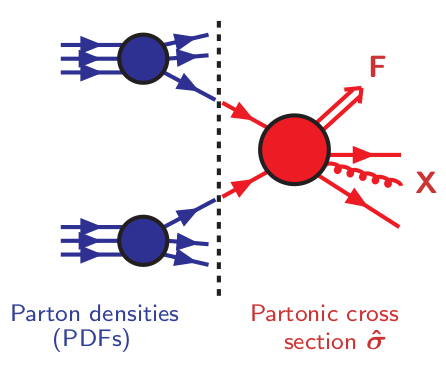
\includegraphics[width = 5 cm]{plots/factorization_3.png}
		\end{figure}
	
	\end{columns}
	
	\begin{equation}
		\hat{\sigma} = \sigma^{\texttt{Born}} \Bigg( 1 +
		\frac{\alpha_{s}}{2\pi} \sigma^{(1)} + 
		\Big(\frac{\alpha_{s}}{2\pi}\Big)^{2} \sigma^{(2)} + 
		\Big(\frac{\alpha_{s}}{2\pi}\Big)^{3} \sigma^{(3)} + ... \Bigg) \nonumber
	\end{equation}
	
	Leading order predictions can strongly depend on the renormalization and factorization scales $\rightarrow$ {\color{red}Need higher order corrections}

\end{frame}

% Dealing with divergences
\begin{frame}

	\center{\color{blue}Resummation in QCD}

\end{frame}

% Higher order corrections
\begin{frame}

	\frametitle{Resummation in QCD}
	\framesubtitle{Higher order corrections}
	\begin{columns}
	
	\column{0.45\textwidth}
	
	\begin{enumerate}
		\item Higher order corrections are {\color{red}not an easy task} due to {\color{red} infrared (IR) singularities}
		\item Soft and collinear singularities
		\item Impossible direct use of numerical techniques
	\end{enumerate}
	
	\column{0.45\textwidth}
	\begin{figure}[!htb]
		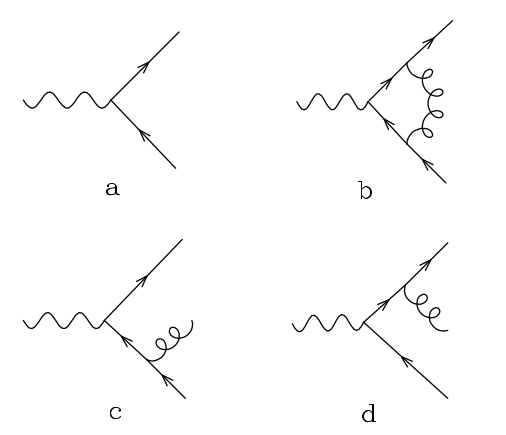
\includegraphics[width = \linewidth]{plots/qcd_corrections.png}
	\end{figure}
	
	\end{columns}

\end{frame}

% q_{\perp} resummationI
\begin{frame}

	\frametitle{Resummation in QCD}
	\framesubtitle{$q_{\perp}$ resummation}
	
	Produce a final state from hadron collisions and study the $q_{\perp}$ distribution 
	
	\begin{columns}
	\column{0.45\textwidth}
	
	$h_{1}(p_{1}) + h_{2}(p_{2}) \longrightarrow F(M, {\color{red}q_{\perp}}) + X$

	\column{0.55\textwidth}
	
	\begin{figure}
		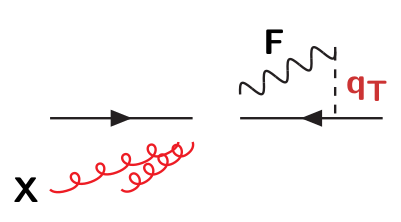
\includegraphics[width = 4cm]{plots/qT_diagram.png}
	\end{figure}

	\end{columns}

	\begin{figure}
		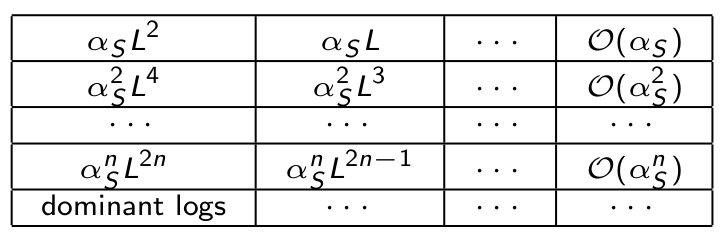
\includegraphics[width = 7cm]{plots/qT_logs_table.png}
	\end{figure}

	Truncated fixed order predictions $\rightarrow$ {\color{red}divergent $\alpha_{s}^{n}\ln^{m}(M^{2}/q_{\perp}^{2})$ appear}.

\end{frame}

% Resummation in QCD II
\begin{frame}

	\frametitle{Resummation in QCD}
	\framesubtitle{$q_{\perp}$ resummation}

	Replace partonic $q_{\perp}$ distribution as follows
	
	\begin{equation}
		\frac{d\hat{\sigma}_{ab}}{dq_{\perp}^{2}} \rightarrow 
		\Bigg[ \frac{d\hat{\sigma}^{\textrm{(res.)}}_{ab}}{dq_{\perp}^{2}} \Bigg]_{\textrm{l.a.}} + 
		\Bigg[ \frac{d\hat{\sigma}^{\textrm{(fin.)}}_{ab}}{dq_{\perp}^{2}} \Bigg]_{\textrm{f.o.}} \nonumber
	\end{equation}

	such that
	\begin{align}
		\int dq_{\perp}^{2} \frac{d\hat{\sigma}^{\textrm{(res.)}}_{ab}}{dq_{\perp}^{2}} &\sim \sum \alpha_{s}^{n} \log^{m} \frac{M^{2}}{Q_{\perp}^{2}} \textrm{\quad for \quad} q_{\perp} \rightarrow 0 \nonumber \\
		\int dq_{\perp}^{2} \frac{d\hat{\sigma}^{\textrm{(fin.)}}_{ab}}{dq_{\perp}^{2}} &\sim 0 \nonumber \textrm{\quad for \quad} q_{\perp} \rightarrow 0
	\end{align}

\end{frame}

% Resummation in QCD III
\begin{frame}

	\frametitle{Resummation in QCD}
	\framesubtitle{$q_{\perp}$ resummation}
	
	Resummation holds in impact parameter space $b$
	\begin{equation}
		\frac{d\hat{\sigma}_{ab}^{\textrm{res.}}}{dq_{\perp}^{2}} = \frac{M^{2}}{\hat{s}} \int db \; \frac{b}{2} \; J_{0}(b q_{\perp}) \; {\color{red} \mathcal{W}_{ab}(b, M)} \nonumber
	\end{equation}
	
	Which is expressed in Mellin space (with respect to $z = M^{2}/\hat{s}$)
	\begin{equation}
		{\color{red} \mathcal{W}_{N}(b, M) = \mathcal{H}_{N}(\alpha_{s}) \times exp\{\mathcal{G}_{N}(\alpha_{s}, L)\}} \quad\textrm{being}\quad L \equiv \log(M^{2}b^{2}) \nonumber
	\end{equation}

	\begin{itemize}
		\item Resummed effects exponentiated in a universal Sudakov factor
		\item Process-dependence factorized in the hard factor
	\end{itemize}

	
\end{frame}

% HTurbo
\begin{frame}

\center{\color{blue}HTurbo: Fast predictions for Higgs production}

\end{frame}

% HqT and HRes
\begin{frame}

	\frametitle{HqT and HRes}
	\framesubtitle{Predictions for Higgs $q_{\perp}$ distribution}
	
	\begin{columns}
		
		\column{0.45\textwidth}
			
			\begin{itemize}
				\item HqT and HRes {\color{blue}[de Florian, G.F., Grazzini, Tommasini]} produce $q_{\perp}$ distributions
				\item Higher order corrections require {\color{red}high computation times}
				\item Codes producing fast predictions are needed for precision era of the LHC
			\end{itemize}

		\column{0.45\textwidth}
	
		\begin{figure}
			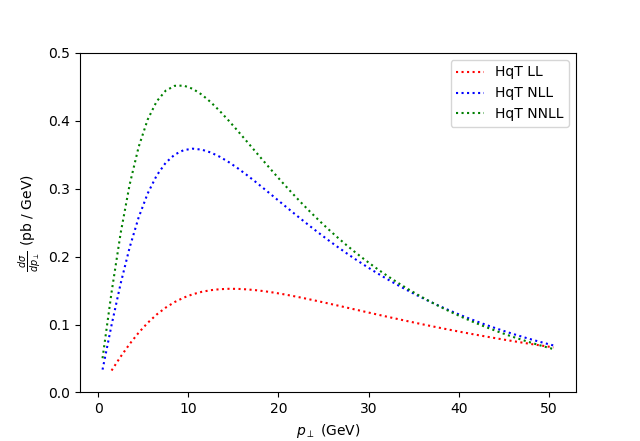
\includegraphics[width = 7 cm]{plots/higgs_qt_all.png}
		\end{figure}		
			
	\end{columns}

\end{frame}

% DYturbo II
\begin{frame}

\frametitle{HTurbo}
\framesubtitle{Starting point DYTurbo}
	
	Start from \textbf{DYTurbo} [Camarda et al.] ref. at {\color{blue} \href{https://arxiv.org/abs/1910.07049}{1910.07049}}, producing $q_{\perp}$ distribution fro Drell-Yan ($q\bar{q} \rightarrow l^{+}l^{-}$)
	
	\begin{itemize}
		\item Set LO amplitude to be $gg \rightarrow H$
		\item Set Sudakov and Hard coefficients for Higgs production
		\item Compare with \textbf{HRes} and \textbf{HqT}
	\end{itemize}

\end{frame}

% DYturbo II
\begin{frame}

	\frametitle{HTurbo}
	\framesubtitle{Starting point DYTurbo}
	
	\begin{itemize}
		\item Set LO amplitude to be $gg \rightarrow H$
		\item Set Sudakov and Hard coefficients for Higgs production
		\item Compare with \textbf{HRes} and \textbf{HqT}
	\end{itemize}
	
	\begin{align}
		\mathcal{G}(\alpha_{s}, L) &= L\;g^{(1)}(\alpha_{s}L) + g^{(2)}(\alpha_{s}L) + \frac{\alpha_{s}}{\pi}g^{(3)}(\alpha_{s}L) + ... \nonumber \\
		\mathcal{H}(\alpha_{s}) &= 1 + \frac{\alpha_{s}}{\pi}\mathcal{H}^{(1)} + \Big(\frac{\alpha_{s}}{\pi}\Big)^{2}\mathcal{H}^{(2)} + ...  \nonumber
	\end{align}
	
	\begin{columns}
		
		\column{0.45\textwidth}

		Build predictions up to NNLO
	
		\column{0.45\textwidth}
		
		\begin{align}
			&\textrm{LL} (\sim \alpha_{s}^{n}L^{n+1}): g^{(1)}, \hat{\sigma}^{(0)} \nonumber \\
			&\textrm{NLL} (\sim \alpha_{s}^{n}L^{n}): g^{(2)}, \mathcal{H}^{(1)} \nonumber \\
			&\textrm{NNLL} (\sim \alpha_{s}^{n}L^{n-1}): g^{(3)}, \mathcal{H}^{(2)} \nonumber
		\end{align}
		
	\end{columns}

\end{frame}

% Results LL
\begin{frame}
	
	\frametitle{Results}
	\framesubtitle{Comparison HTurbo and HqT}
	
	\begin{figure}
		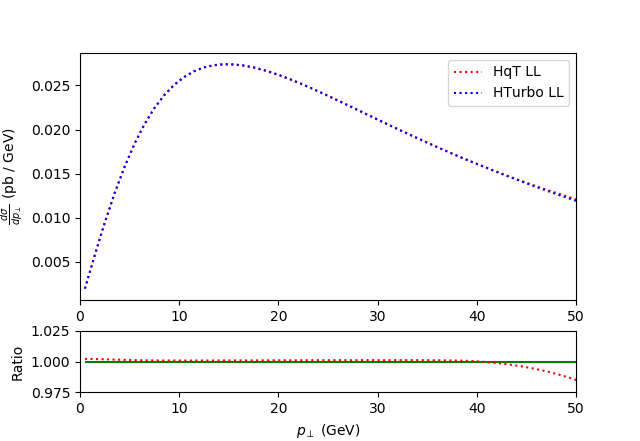
\includegraphics[width = 8cm]{plots/hturbo_LL.png}
	\end{figure}
	
	\begin{itemize}
		\item HTurbo produces qt distributions that match HRes and HqT
		\item Excellent numerical agreement up to the 1/1000
	\end{itemize}

\end{frame}

% Results NLL
\begin{frame}

	\frametitle{Results}
	\framesubtitle{Comparison HTurbo and HqT}
	
	\begin{figure}
		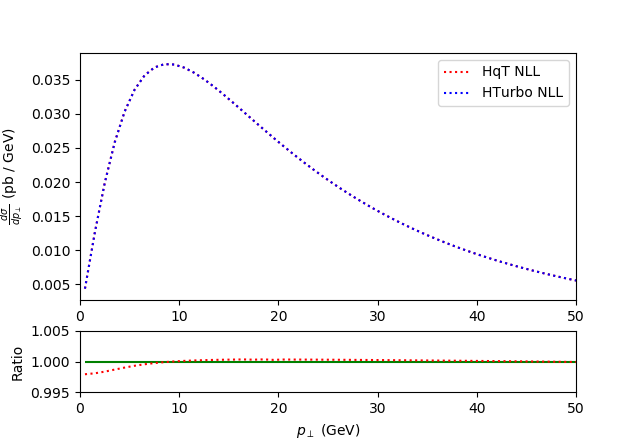
\includegraphics[width = 8cm]{plots/hturbo_NLL_noevol.png}
	\end{figure}
	
	\begin{itemize}
		\item Excellent numerical agreement up to the 1/1000
		\item Perfect agreement when switching off PDF evolution
	\end{itemize}

\end{frame}

% Results NNLL
\begin{frame}

	\frametitle{Results}
	\framesubtitle{Comparison HTurbo and HqT}
	
	\begin{figure}
		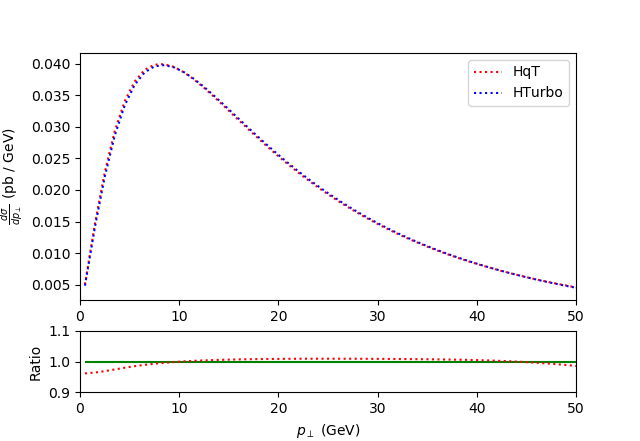
\includegraphics[width = 8cm]{plots/hturbo_NNLL_f2only2.png}
	\end{figure}
	
	\begin{itemize}
		\item Excellent numerical agreement up to the 1/1000
		\item Perfect agreement when switching off PDF evolution
	\end{itemize}

\end{frame}

% Results NNLL
\begin{frame}
	
	\frametitle{Results}
	\framesubtitle{Comparison HTurbo and HqT}
	
	\begin{figure}
		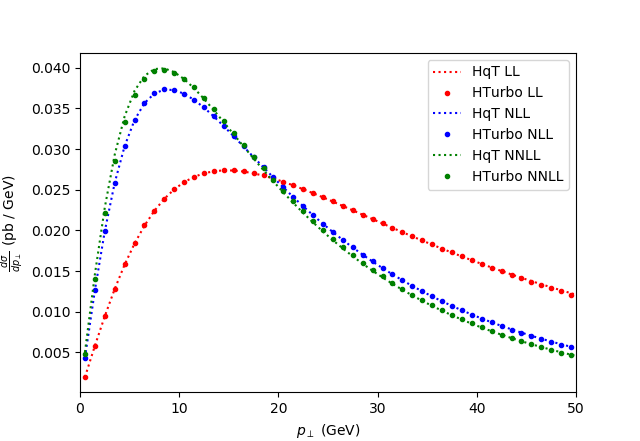
\includegraphics[width = 8cm]{plots/hturbo_all_noevol.png}
	\end{figure}
	
	\begin{itemize}
		\item Excellent numerical agreement up to the 1/1000
		\item Perfect agreement when switching off PDF evolution
	\end{itemize}

\end{frame}

% Conclusions
\begin{frame}
	
	\frametitle{Summary $\&$ Conclusions}

	\vspace{2.0 cm}
	
	\begin{enumerate}
		\item Fast predictions are required towards the precision era of the LHC
		\item HTurbo produces qt distributions that perfectly match HRes and HqT
		\item Predictions by HTurbo are much faster than any of the existing codes
		\item Next steps: Implement PDF evolution N3LO distributions

	\end{enumerate}

	\vspace{2.0 cm}

\end{frame}

% Conclusions
\begin{frame}

\center {\color{blue}Thank you!}

	\begin{figure}
		
\includegraphics[width = 4 cm]{plots/thinking.png}
	\end{figure}		


{\small \color{blue} This project has received funding from the European Union$'$s Horizon 2020 research and innovation program under grant agreement No 740006.}

\end{frame}


\end{document}